\chapter{Expressing Parallelism}
\label{chapter:exposing_parallelism}

Multimedia codecs such as MPEG-2 demand high performance because of throughput
requirements. An online encoder or decoder must be capable of realtime performance,
which can be as high as 60 fps. An offline encoder is less constrained but minimizing
total runtime is still a concern. Since traditional CPU clock scaling has ended,
meeting throughput demands requires parallel scalable implementations. 
Critical to these implementations is the compiler's ability to detect parallelism
in a program specification. 
This section examines how parallelism was successfully 
realized in the MPEG-2 codecs and how the StreamIt language made this task easy. The 
parallelism discussed in this section is exposed through the stream graph 
topology rather than by changing any underlying algorithms. This section ignores 
parallelizing MPEG-2 codecs across GOPs; since GOPs are coded independently, 
this is embarrassingly parallel and trivial. I also include proof of 
concept results showing that the StreamIt implementation scales on multicore
architectures.

\section{Splitjoins Express Data Parallelism}

One particularly noteworthy aspect of splitjoins is the ability to define 
their internal topology using the for-loop construct. The for-loop, unrolled at 
instantiation time, makes the degree of parallelism and the stream topology
itself parameterizable. 
This feature makes it easy for the programmer to concisely express a data parallel 
computation. The code responsible for channel upsampling, shown in 
Figure~\ref{fig:upsamplecode}, expresses a massively data parallel computation in 
this way. 

\section{Hierarchical Streams Expose High Degrees of Parallelism}
\label{sec:2d_dct}

\begin{figure}[h]
  \begin{center}
    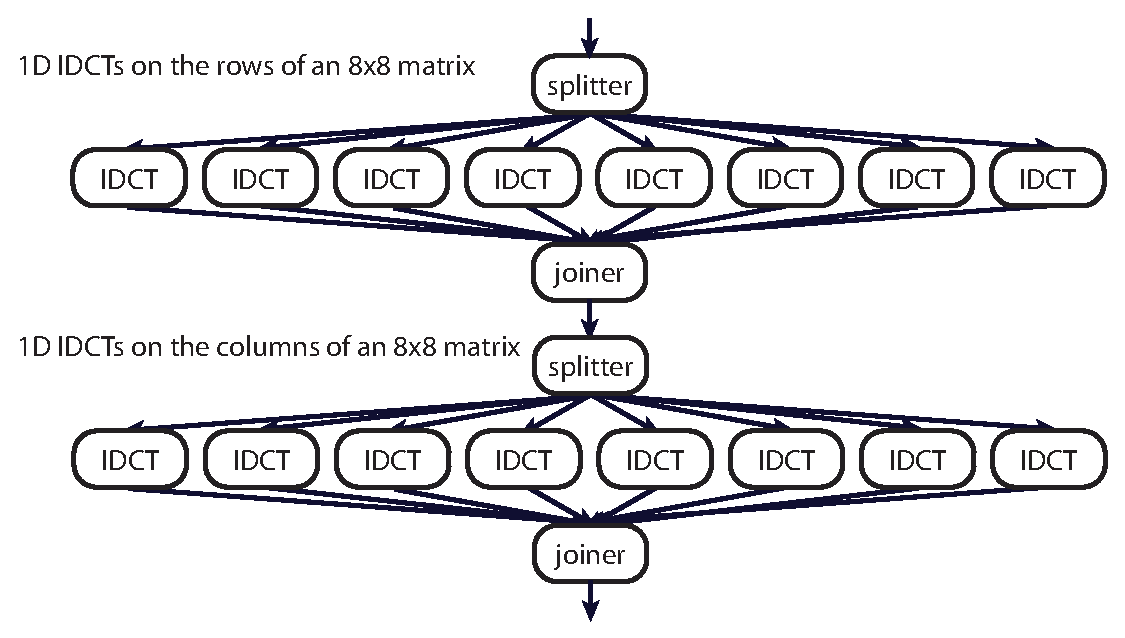
\includegraphics[scale=0.6, angle=0]{./dct_block.eps}
    \caption{Subgraph for a fine grained 2D inverse DCT.}
    \label{fig:decoder-sj-graph}
  \end{center}
\end{figure}

\begin{figure}[h]
  \begin{center}
    \begin{minipage}{4in}
      \begin{small}
        \begin{verbatim}
float->float pipeline IDCT_2D(int N) {
    // perform N 1D-IDCTs in parallel in the X direction
    add splitjoin {
        split roundrobin(N);
        for (int i = 0; i < N; i++)
            add IDCT_1D(N);
        join roundrobin(N);
    }
    // perform N 1D-IDCTs in parallel in the Y direction
    add splitjoin {
        split roundrobin(1);
        for (int i = 0; i < N; i++)
            add IDCT_1D(N);
        join roundrobin(1);
    }
}

float->float filter IDCT_1D(int N) {
    float[N][N] coeff = { ... };
       
    work pop N push N {
        for (int x = 0; x < N; x++) {
            float product = 0;
            for (int u = 0; u < N; u++)
                product += coeff[x][u] * peek(u);
            push(product);
        }
        for (int x = 0; x < N; x++) pop();
    }
}
        \end{verbatim}
      \end{small}
    \end{minipage}
  \end{center}
  \caption{StreamIt code for the fine grained 2D inverse DCT subgraph.}
  \label{fig:decoder-sj}
\end{figure}

\begin{figure}[h]
  \begin{center}
    \begin{minipage}{4in}
      \begin{small}
        \begin{verbatim}
// global variable
float coeff[64] = { ... };
      
void IDCT_2D(float* block) {
    int i, j, u;
    float product;
    float tmp[64];
        
    // 1D DCT in X direction
    for (i = 0; i < 8; i++)
        for (j = 0; j < 8; j++) {
            product = 0;
            for (u = 0; u < 8; u++)
                product += coeff[u][j] * block[8*i + u];
            tmp[8*i + j] = product;
        }

    // 1D DCT in Y direction
    for (j = 0; j < 8; j++)
        for (i = 0; i < 8; i++) {
            product = 0;
            for (u = 0; u < 8; u++)
                product += coeff[u][i] * tmp[8*u + j];
            block[8*i + j] = product;
        }
}
        \end{verbatim}
      \end{small}
    \end{minipage}
  \end{center}
  \caption{C code for 2D inverse DCT calculation using two 1D transforms.}
  \label{fig:idct_creference}
\end{figure}

Hierarchical constructs provide a convenient and natural
way to represent parallel computation. 
Figure~\ref{fig:decoder-sj-graph} shows a parallel
implementation of the 2D IDCT using 1D IDCTs. This
implementation is both data parallel (within the rows and columns) and
pipeline parallel (between the rows and columns). 
The StreamIt code for this 2D IDCT appears in Figure~\ref{fig:decoder-sj}.
A straightforward C implementation of a computationally equivalent
IDCT is shown in Figure~\ref{fig:idct_creference}. Note that
the code structure is similar to the StreamIt version, although it does 
not explicitly expose the parallelism; the compiler must perform loop
and dependency analysis to enable parallelism.
The C code also requires explicit array index management, such as the 
expressions $\texttt{block[8*i+u]}$ and $\texttt{tmp[8*i+j]}$, which are
notably absent in the StreamIt code. 
The splitter and joiner in StreamIt free the programmer from
tedious indexing operations, which also enables the compiler to
understand and optimize the buffer management~\cite{sermulins05lctes}.
The StreamIt implementation is also parameterized such that it is
trivial to adjust the size of the IDCT.

\section{Parallelizing Motion Prediction}
\label{sec:parallelmotion}

Motion prediction, in both the decoder and encoder, represents a significant fraction of the 
computational effort, and is amenable to data parallelism. Because each block in a 
picture has an associated set of motion vectors, motion prediction filters 
express a block-level transformation, and predictions for blocks may be formed in 
parallel. However, the act of forming the prediction requires a filter have access to 
full reference pictures. A parallel implementation of motion prediction will either lead 
to redundant copies of the reference pictures or the necessity for motion prediction 
threads to share a global read only memory space where the reference pictures can be stored. 
A parallel motion prediction algorithm is easy to express in StreamIt and exposes the 
necessary information so that the compiler can provide a shared-memory storage for the 
reference pictures.

\begin{figure}[h]
  \begin{center}
    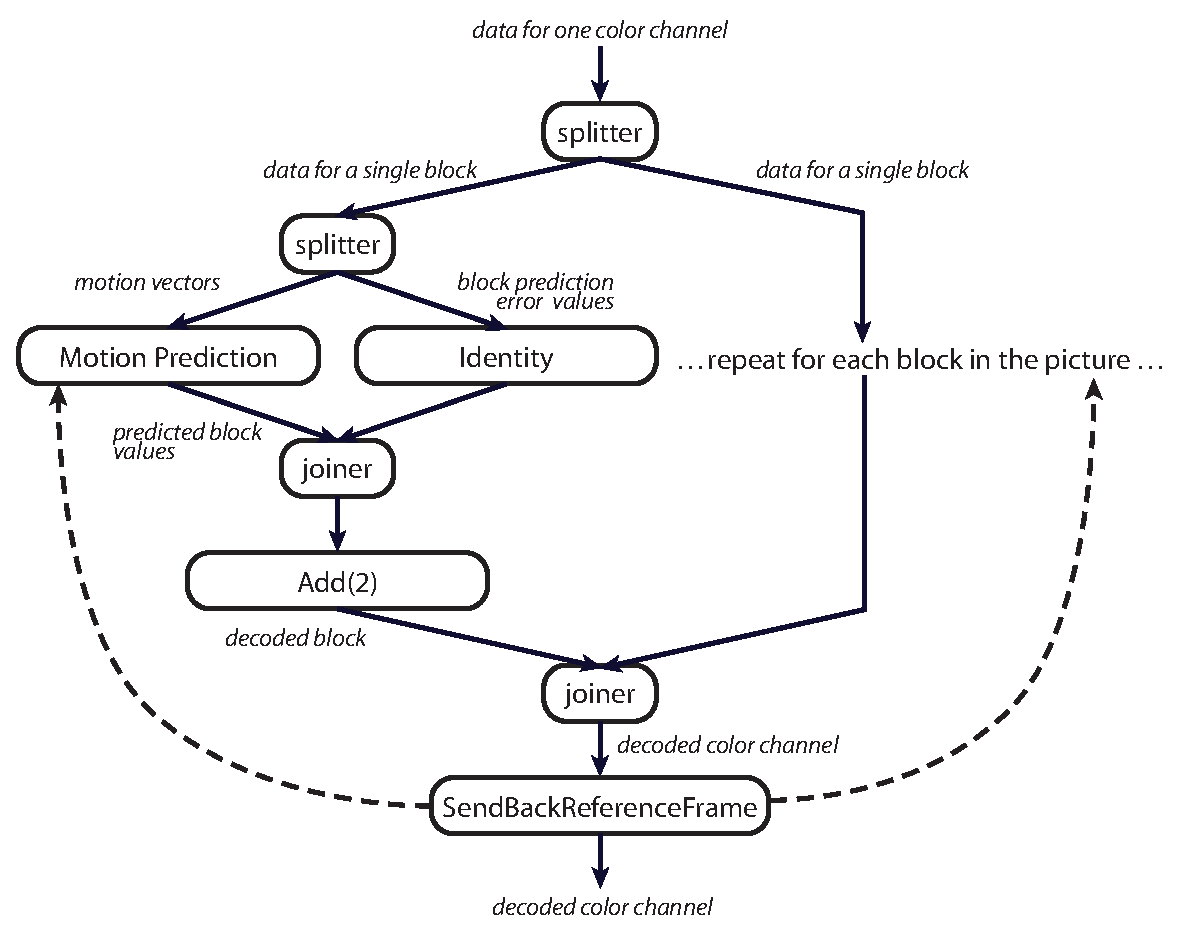
\includegraphics[scale=0.7, angle=0]{./motion_compensation.eps}
    \caption{Stream topology for motion compensation of a single color channel.}
    \label{fig:motion_prediction_parallel}
  \end{center}
\end{figure}

Figure~\ref{fig:motion_prediction_parallel} shows the StreamIt pipeline responsible for 
motion compensation of a single color channel in the decoder. All blocks in a given 
picture are motion predicted in parallel, with a set of block prediction error values 
and motion vector information sent to each motion prediction filter. Each data set then 
has its block coefficients (which need no processing) and the motion vectors splitup, 
sending the motion vectors to the filter that actually does the work of computing the 
predicted block using the motion vector offsets. The predicted block output is added 
to the block prediction error to form the original block, and all blocks are 
interleaved in the data streams. The final filter in the stream graph is responsible for 
communicating this fully decoded picture back to the motion prediction filters. It 
does this by sending upstream messages containing the reference picture data.

Note the cleanliness of this parallel implementation: 
a programmer could manually change the number of blocks 
decoded in parallel and similarly, the compiler can 
automatically fuse filter instances to match the target 
hardware. 
Note also that the reference pictures needed 
by the motion compensation filter and the picture type 
data needed by both the motion compensation and 
reference frame sending filters are naturally expressed using 
messaging. Finally, note that the motion compensation filters
only need to form predictions using their available reference
pictures and a separate filter can make sure they access
the correct references.

As mentioned previously, the one potential drawback of this
scheme would be if each instance of the motion prediction 
filter required its own instance of the reference picture 
data. However, a simple optimization allows the compiler to 
detect that these motion prediction filters only use these 
reference pictures in a read-only context and they may be 
stored in a global address space. Suppose that a filter 
receives a message containing a nugget of data $X$. If a 
compiler can detect that the filter never modifies $X$, 
it can place a copy in a shared memory space and give the 
filter a reference to $X$. Whenever a new message is 
received, it simply gives the filter a new reference to the 
data in a different part of the shared memory space. If 
a filter modifies $X$ or the compiler cannot detect 
that the filter uses $X$ immutably, it must give the 
filter a copy of the message in its own address space. Some 
kind of reference count or garbage collection mechanism 
must be associated with data stored in the global space 
so that the memory can be freed or reused once no filters 
can access the data.

The read-only analysis and associated space saving 
optimization can be performed by the compiler automatically. 
This enables program implementations to use a global 
reference space, even though the language need not provide 
this feature. I have tested a prototype of this optimization 
in the StreamIt Java library, where garbage collection is 
easily handled, and verified that it works.

\section{Improving Decoder Parallelization}
\label{section:super_parallel}

Most MPEG-2 decoder implementations make spatial decoding 
precede temporal decoding, but nothing in the specification 
or decoding algorithms require this. To achieve a higher degree of 
parallelization, one would want to generate the predictions for a 
block in parallel with the spatial interpretation of the block 
coefficients. This has been tried with success in a hardware based 
implementation~\cite{schneider99spec}. Only near the final output 
stage must the prediction and spatial data be summed and the output 
generated.

\begin{figure}
  \begin{center}
    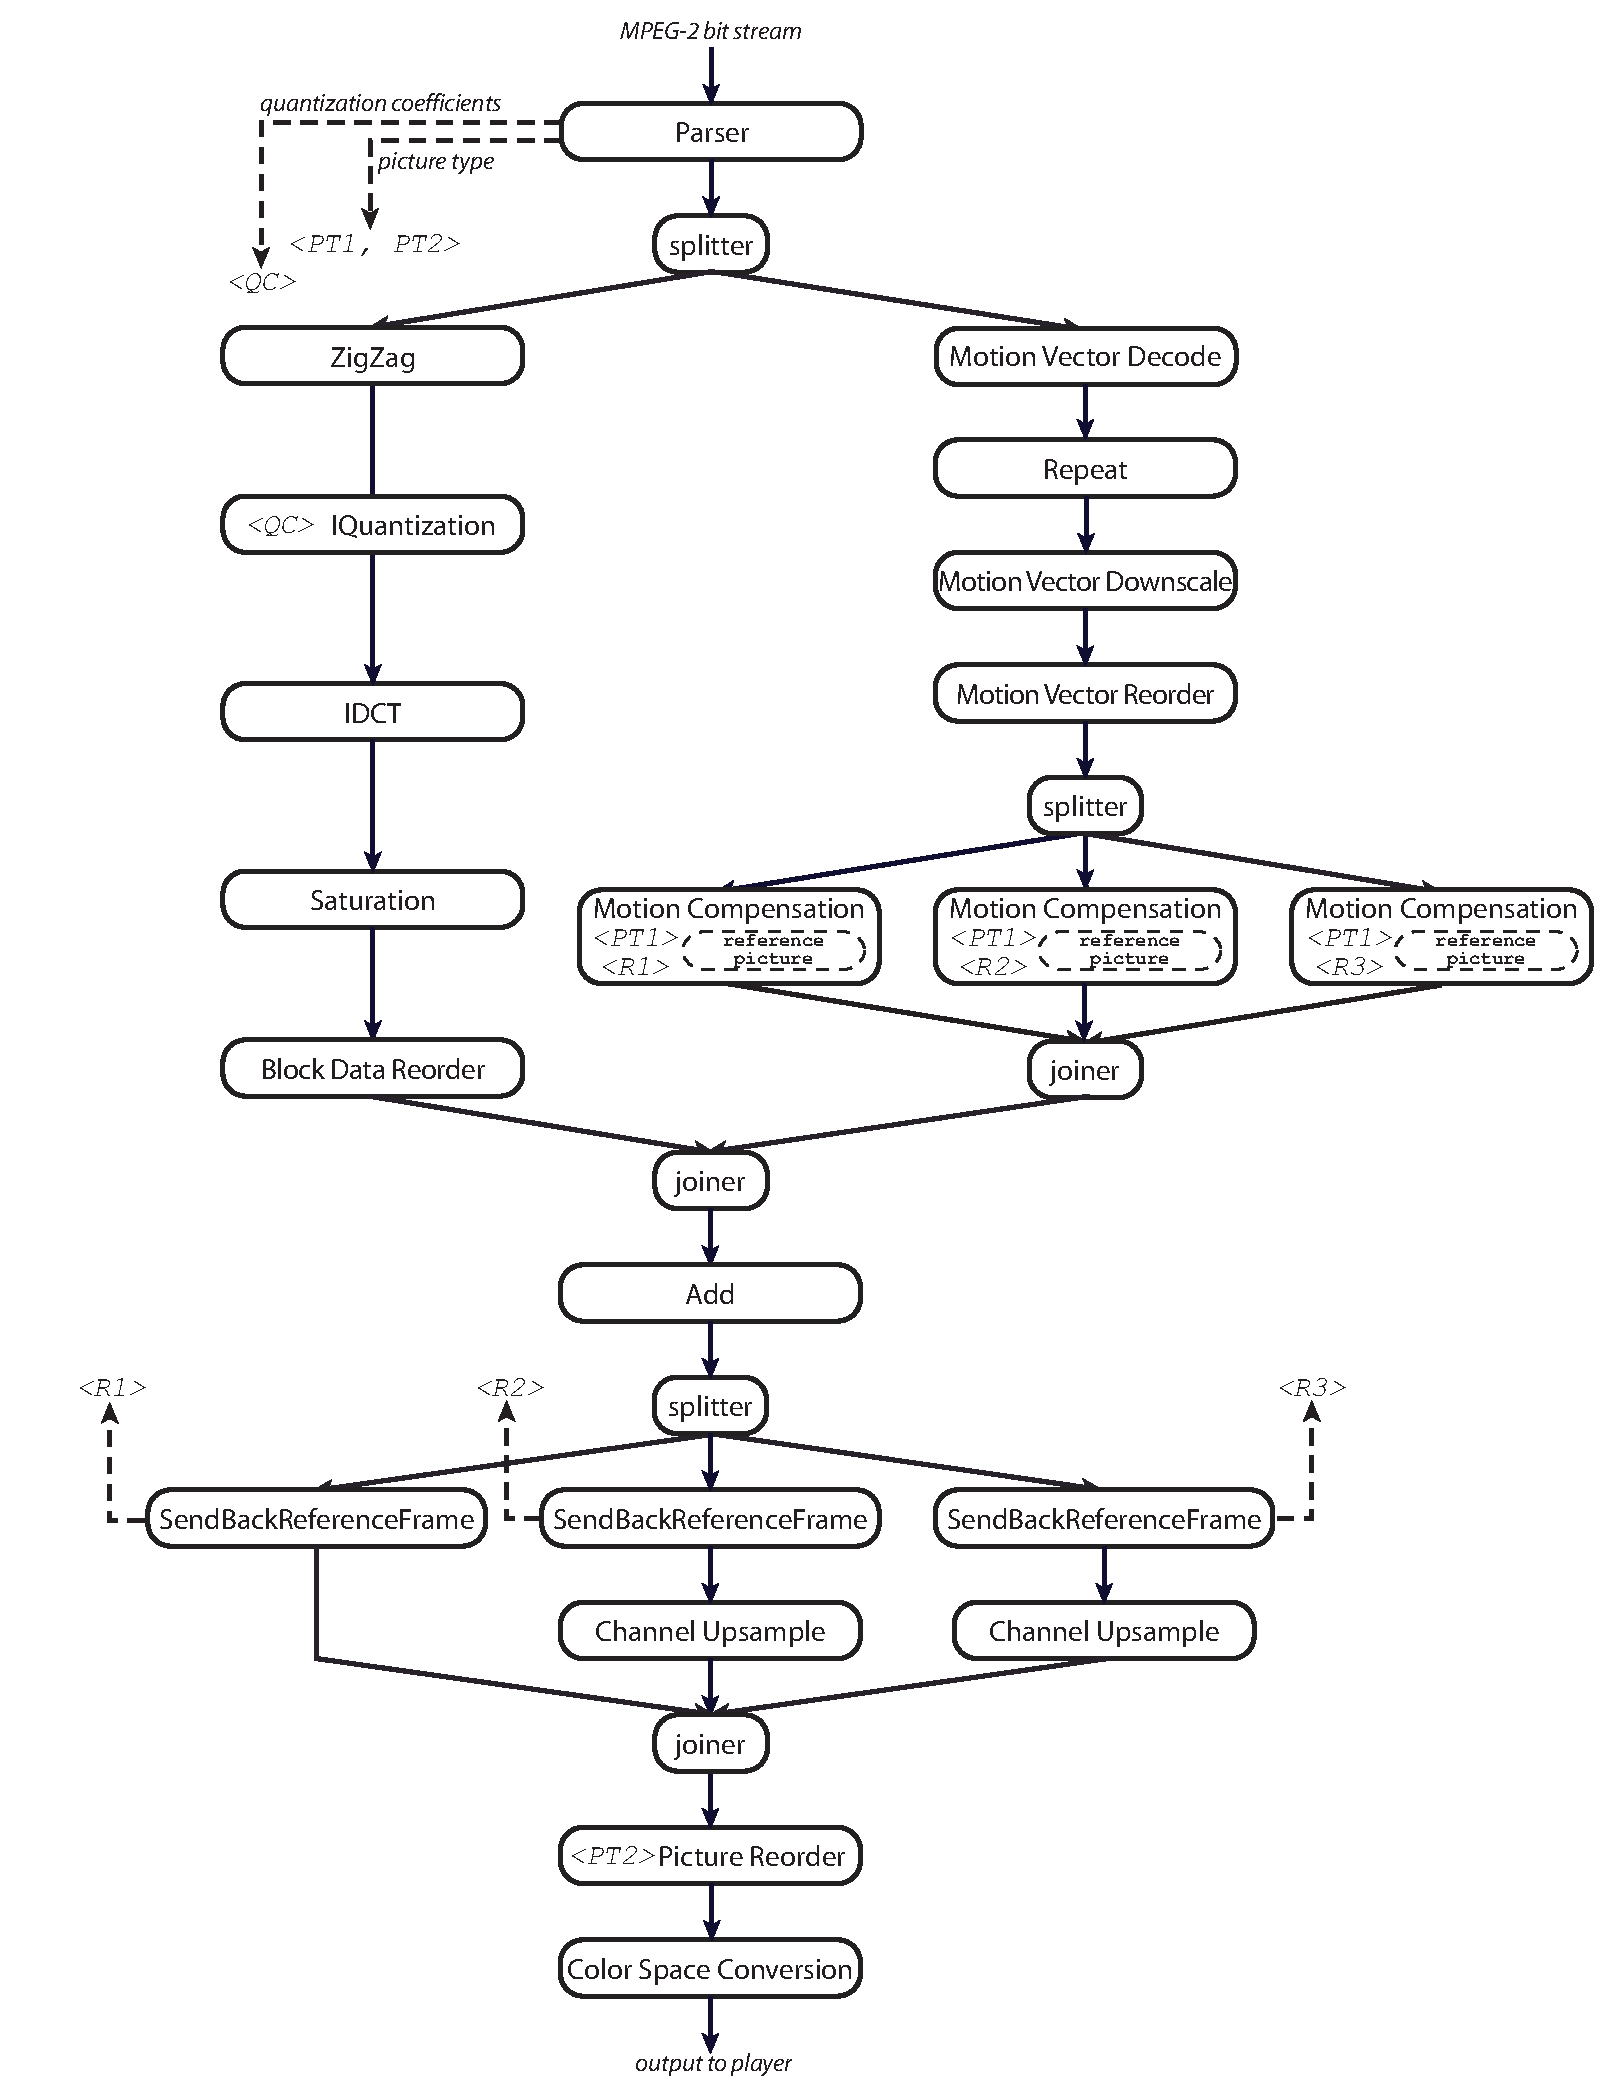
\includegraphics[scale=0.40, angle=0]{./decoder_total_parallelization.eps}
    \caption{Exposing parallelism between spatial and temporal decoding in an MPEG-2 decoder.}
    \label{fig:total_parallelization_vs_old_way}
  \end{center}
\end{figure}

I previously showed a block diagram for the MPEG-2 decoder 
in StreamIt (in Figure~\ref{fig:dec-with-code}). This diagram 
represents both a straightforward block specification and a program 
definition derived from the specification.  
Figure~\ref{fig:total_parallelization_vs_old_way} shows 
an alternative block diagram for an MPEG-2 decoder. This 
alternative diagram shows a block diagram that an MPEG-2 expert will decide 
upon\footnote{The original diagram represents the program structure 
I chose a month after originally familiarizing myself with the 
MPEG-2 specification. The new diagram represents the program 
structure I chose 8 months later after extensive familiarity 
with the specifications and implementations.}. These two block 
diagrams contain the same functional transformations. For an 
ideal language, a clean and malleable implementation of the 
original block specification in Figure~\ref{fig:dec-with-code} 
could easily be modified to expose the greater degree of 
parallelism present in the expert's block structure in 
Figure~\ref{fig:total_parallelization_vs_old_way}.

Because StreamIt preserves block structure in the program 
definition this transformation is easily accomplished. I have 
implemented the alternate decoder, using exactly the same 
filters as those used in the original decoder implementation. 
These two implementations are functionally equivalent, 
generating the same output across test cases. The only 
changes in the code are to the nested hierarchical container 
topologies that dictate the decoder stream graph. The ease 
with which a programmer can expose greater parallelism by 
merely changing the stream topology points to the 
usefulness of stream based languages for parallel program 
implementations.

\section{Performance Results}

This section provides performance results showing how StreamIt 
enables a compiler to provide scalable performance on MPEG-2 
codec implementations. A need for new language features previously 
mentioned in this thesis prevents the compilation of a full 
decoder or encoder\footnote{An intermediate Java library output 
from the compiler allows me to verify correctness of StreamIt code. This target is 
not performance oriented.}. 
Execution and evaluation of the complete MPEG-2 decoder and encoder stream graphs 
is a current focus of the StreamIt group.
Here I consider the spatial decoding subgraph, 
which represents up to a third of the total computation
in the decoder~\cite{iwata98coarse}.
I have extracted the 
spatial decoding code from the StreamIt and C decoder implementations
so that it can be compiled and run on a performance oriented target.

\begin{figure}[h]
 \begin{center}
  \begin{tabular}{|l|c|c|}
\hline
Granularity & Nodes in IDCT & Nodes in Graph\\
\hline
Coarse & 2 & 8 \\
Intermediate & 11 & 17\\
Fine & 20 & 26\\
\hline
  \end{tabular}
  \end{center}
 \caption{Three versions of the spatial decoding stream graph and their granularities.}
 \label{table:decoding_graphs}
\end{figure}

I use three versions of the StreamIt spatial decoding stream graph with
differing granularities. The granularities are changed by altering the subgraph
for the 8x8 IDCT. Figure~\ref{table:decoding_graphs} lists the number of nodes
(filters, splitters, and joiners), contained in the stream graph for each
of the three versions.
Each version contains \texttt{Source}, \texttt{ZigZag}, 
\texttt{InverseQuantization}, \texttt{Saturation}, \texttt{MismatchControl}, and
\texttt{Sink} filters. The coarse grained IDCT uses 2 filters for the IDCT: 
a \texttt{Rows\_iDCT} and a \texttt{Columns\_iDCT} filter. The fine grained
IDCT is expressed with 16 1D IDCTs and two splitjoins as described 
in Section~\ref{sec:2d_dct}. 
The intermediate IDCT uses the coarse \texttt{Rows\_iDCT} filter for the row
transformation and the fine grained column transformation with 8 1D IDCTs.

The performance evaluation is carried out on the Raw architecture
\cite{taylor:micro:2002, taylor:isca:2004}.
The Raw architecture is representative of the industry shift to multicore
embedded architectures, currently manifested in emerging architectures
such as the Intel Duo, AMD Opteron, and IBM Cell processors.
Raw is a wire-exposed multicore architecture which contains a 2D array of identical,
programmable tiles 
and supports instruction, data, thread, and pipeline parallelism. 
Each tile has a compute processor and a switch processor that
manages communication. The compute processor is composed of an eight-stage
in-order single-issue MIPS-style processor, a four-stage pipelined floating point unit,
a 32kB data cache, and a 32kB instruction cache. 
Tiles are connected by a FIFO queue 
with a 3 cycle near neighbor latency. This interconnect
network provides a mechanism for filters to communicate quickly with each other.
The current Raw prototype is a chip with 16 tiles running at 425Mhz. 
For this thesis, results are gathered using
a cycle-accurate simulator~\cite{taylor:isca:2004} that can model tile configurations
with size
1, 4 (2x2 grid), and 16 (4x4 grid). 

\begin{figure}[p]
  \begin{center}
    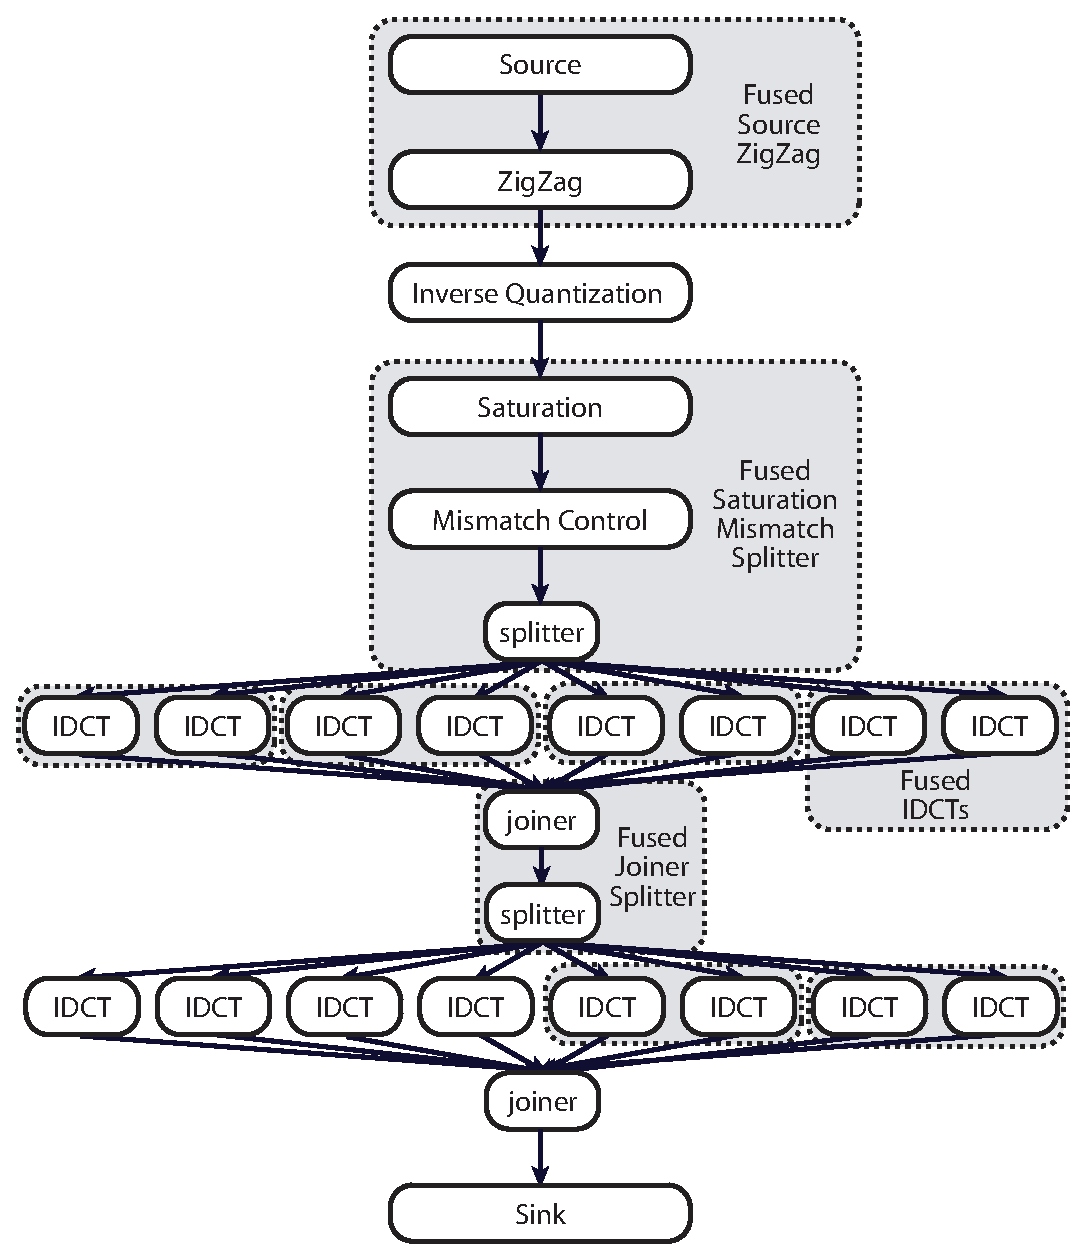
\includegraphics[scale=0.5, angle=0]{./partition.eps}
    \caption{Partitioning the spatial decoding stream graph for 16 tiles of Raw.}
    \label{fig:partition}
  \end{center}
\end{figure}

\begin{figure}[p]
  \begin{center}
    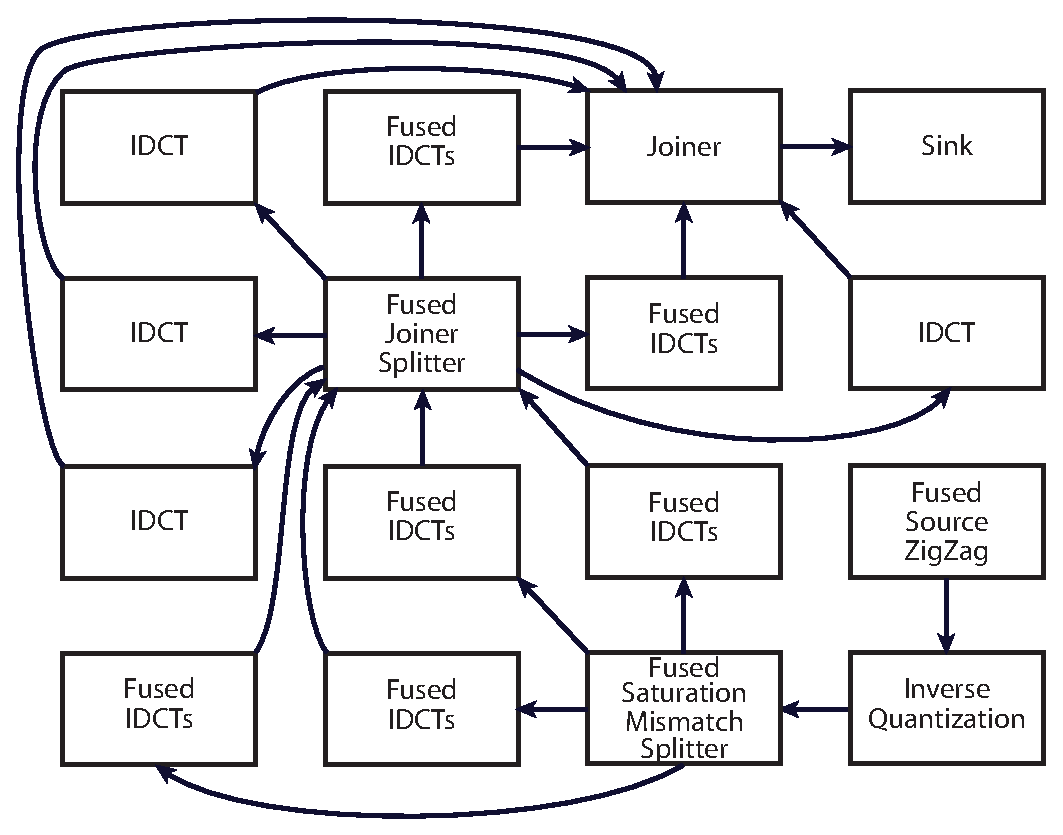
\includegraphics[scale=0.5, angle=0]{./layout.eps}
    \caption{Layout of the fine grained spatial decoding stream graph on the Raw chip.}
    \label{fig:layout}
  \end{center}
\end{figure}

The StreamIt code was compiled to Raw with the StreamIt 
space multiplexing compiler
\footnote{This compiler will soon be
deprecated in favor of a more advanced space-time multiplexing
compiler described in an upcoming paper~\cite{gordon06asplos} 
from the StreamIt group.}
described in~\cite{gordon02asplos}.
The code was compiled at an \texttt{-O1} optimization level, 
which performs loop unrolling by a factor
of 16, scalar replacement, and aggressive constant propagation. 
The StreamIt compiler focusses on achieving
performance by enabling scalable execution on
many tiles. Using the parallelism explicit in the stream graph the compiler
automatically performs task partitioning and layout.
An application should achieve significant speedups as the number of tiles increases.

A brief example illustrating
scheduling and layout follows.
Figure~\ref{fig:partition} shows how the StreamIt
compiler partitions the fine grained 
spatial decoding stream graph for a Raw configuration with 16 tiles.
The compiler adjusts the stream graph granularity by combining
nodes to eliminate buffering between nodes on the same tile. 
The dotted lines in the figure show which nodes in the stream graph have been fused.
After fusion is complete there are the same number of nodes and tiles 
in the stream graph. Figure~\ref{fig:layout}
shows the compiler's layout decision for these nodes on the Raw hardware.

\begin{figure}[t]
  \begin{center}
    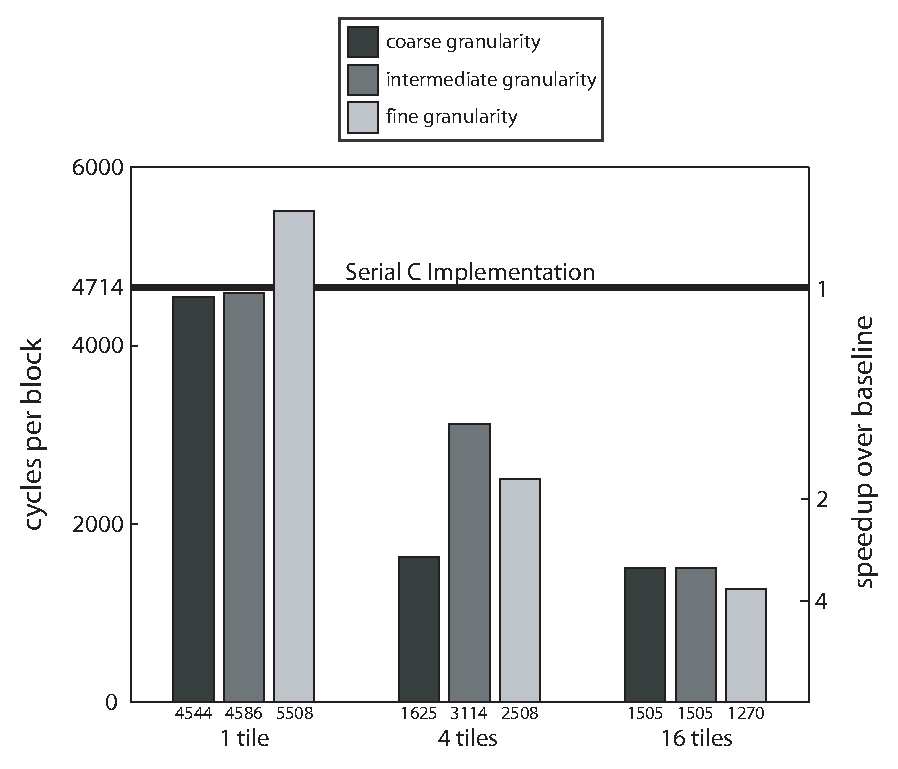
\includegraphics[scale=0.7, angle=0]{./performance_graph.eps}
    \caption{Scalability of StreamIt spatial decoding pipeline against single tile C baseline.}
    \label{fig:performance_results}
  \end{center}
\end{figure}

Figure~\ref{fig:performance_results} shows results for execution of 
the spatial decoding stream graph at three granularities.
The baseline is
the C reference code running on a single tile. 
The C code was compiled with a Raw port of the \texttt{gcc} compiler,
which performs register allocation and list scheduling.
A compiler has a difficult time extracting parallelism from single threaded C code
(hence the need for new programming models); in StreamIt the parallelism
is explicit, so we show performance numbers for multi-tile 
configurations as well. 

Single tile StreamIt performance is roughly equivalent to the
single tile C code. Small variations are explained
by compiler decisions about how to fuse all the filters together. 
When the tile size increases to 4, all versions of the StreamIt
code significantly outperform the C implementation. While 
the coarse grained
version of the StreamIt code outperforms the more fine grained
implementations, an analysis of the compiler's layout decisions suggests
that this result is somewhat anomalous: the compiler is 
getting exceptionally lucky with load balancing. The intermediate
and fine grained versions are more prototypical.
At 16 tiles performance of all stream graphs 
again improves significantly. One 
sees the general trend that decreasing the granularity of
the program enables the compiler to make better layout
decisions and provide higher parallel performance. The best 
performance comes from a fine-grained implementation 
operating on 16 tiles.
